\documentclass[tikz, convert={outfile=\jobname.svg}]{standalone}

\usepackage{tikz-cd}
\usetikzlibrary{fit,positioning}
\usetikzlibrary{matrix,shapes}
\usetikzlibrary{arrows.meta} % 
\usetikzlibrary{arrows}
\usepackage{tikz}

\begin{document}


\begin{figure}
    \centering
    % TODO:["Fix this tikz"]
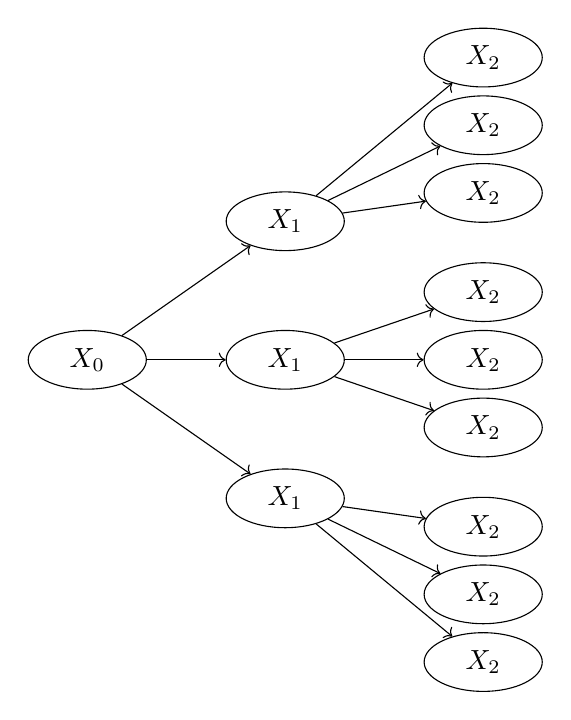
\begin{tikzpicture}[mynode/.style={draw,ellipse, minimum width=1.5cm, minimum height=.8mm}]

\node[mynode] (X_0) {$X_0$};

\node[mynode, right=of X_0] (X_1^2) {$X_1$};
\node[mynode, below=of X_1^2] (X_1^3) {$X_1$};
\node[mynode, above=of X_1^2] (X_1^1) {$X_1$};

\draw[->] (X_0) -- (X_1^1) node[midway,above left] {};
\draw[->] (X_0) -- (X_1^2) node[midway,above] {};
\draw[->] (X_0) -- (X_1^3) node[midway,above] {};

\node[mynode, right=of X_1^2] (X_2^5) {$X_2$};
\node[mynode, above=0.1cm of X_2^5] (X_2^4) {$X_2$};
\node[mynode, below=0.1cm of X_2^5] (X_2^6) {$X_2$};

\node[mynode, above = 0.5cm of X_2^4] (X_2^3) {$X_2$};
\node[mynode, above = 0.1cm of X_2^3] (X_2^2) {$X_2$};
\node[mynode, above = 0.1cm of X_2^2] (X_2^1) {$X_2$};

\node[mynode, below = 0.5cm of X_2^6] (X_2^7) {$X_2$};
\node[mynode, below = 0.1cm of X_2^7] (X_2^8) {$X_2$};
\node[mynode, below = 0.1cm of X_2^8] (X_2^9) {$X_2$};


\draw[->] (X_1^1) -- (X_2^1) node[near end,above left] {};
\draw[->] (X_1^1) -- (X_2^2) node[near end,above ] {};
\draw[->] (X_1^1) -- (X_2^3) node[near end ,above] {};

\draw[->] (X_1^2) -- (X_2^4) node[near end,above left] {};
\draw[->] (X_1^2) -- (X_2^5) node[near end,above ] {};
\draw[->] (X_1^2) -- (X_2^6) node[near end ,above] {};

\draw[->] (X_1^3) -- (X_2^7) node[near end,above left] {};
\draw[->] (X_1^3) -- (X_2^8) node[near end,above ] {};
\draw[->] (X_1^3) -- (X_2^9) node[near end ,above] {};


\end{tikzpicture}

\end{figure}



\end{document}